\documentclass[12pt]{article}
\usepackage[english]{babel}
\usepackage[letterpaper,top=2cm,bottom=2cm,left=3cm,right=3cm,marginparwidth=1.75cm]{geometry}
\usepackage{amsmath}
\usepackage{graphicx}
\usepackage{hyperref}
\title{STAT-UB 103 Homework 8}
\author{Ishan Pranav}
\date{April 23, 2023}
\renewcommand{\thesubsection}{\thesection.\alph{subsection}}
\renewcommand{\theenumi}{\alph{enumi}}
\begin{document}
\maketitle
\section{Learning the mechanics}
\begin{enumerate}
\item See below.
\begin{center}
\begin{tabular}{ccccccc}
$x_i$&&$y_i$&&$x^2_i$&&$x_iy_i$\\\\
7&&2&&49&&14\\
4&&4&&16&&16\\
6&&2&&36&&12\\
2&&5&&4&&10\\
1&&7&&1&&7\\
1&&6&&1&&6\\
3&&5&&9&&15\\\\
$\sum_{i=0}^6{x_i}=24.$&&$\sum_{i=0}^6{y_i}=31.$&&$\sum_{i=0}^6{x^2_i}=116.$&&$\sum_{i=0}^6{x_iy_i}=80.$\\
\end{tabular}
\end{center}
\item\[s^2_{x,y}=\sum^{n-1}_{i=0}{(x_i-\bar{x})(y_i-\bar{y})}\approx -26.2857\dots\]
\item\[s^2_x=\sum^{n-1}_{i=0}{(x_i-\bar{x})^2}\approx 33.7143\dots\]
\item\[b_1=\frac{s^2_{x,y}}{s^2_x}\approx -0.7797\dots\]
\item\[\bar{x}\approx 3.4286\dots\]
\[\bar{y}\approx 4.4286\dots\]
\item\[\bar{y}=b_1\bar{x}+b_0.\]

\[b_0=\bar{y}-b_1\bar{x}\approx 7.1017\dots\]
\item\[\hat{y}=b_1x+b_0=-0.7797x+7.1017.\]
\end{enumerate}
\section{Forecasting movie revenues with Twitter}
\[b_1=0.078767\dots\]
Assuming that movie revenue and tweet rate are linearly related, we estimate a movie's opening weekend revenue increases by an average of 7,876,700 dollars as the tweet rate for the movie increases by an average of 100 tweets per hour.
\section{Congress voting on women's issues}
Let $y$ represent a legislator's American Association of University Women score as a function of the number of daughters ($x$) that the legislator has.

\[y_i=\beta_1x_i+\beta_0+\epsilon_i.\]

\begin{enumerate}
\item If it is true that having a daughter influences voting on women's issues, the sign of $\beta_1$ will be positive. A positive linear coefficient ($\beta_1$) indicates a positive linear relationship.
\item
\[n=434.\]
\[\nu=n-2=432.\]
\[b_1=0.27.\]
\[s_{b_1}=0.74.\]
\[t^*=F^{-1}_{432}(0.025)\approx 1.9655\dots\]

We can be ninety-five-percent confident that the true value of $\beta_1$ is in the interval:
\[(-1.18,1.72)\]

\end{enumerate}
\section{RateMyProfessors.com}
Let $y_i$ represent the student evaluation of teaching and $x_i$ represent the RateMyProfessors.com rating.
\[n=426.\]
\[r_{x,y}=0.68.\]
\begin{enumerate}
\item Let $\beta_1$ represent the linear coefficient of the RateMyProfessors.com rating, $\beta_0$ represent the constant coefficient, and $\epsilon_i$ represent the error term.
\[y_i=\beta_1x_i+\beta_0+\epsilon_i.\]
\item The sample correlation of 0.68 indicates a strong positive linear relationship between the RateMyProfessors.com rating and the student evaluation of teaching. Students who rate their professors highly on RateMyProfessors.com also tend to give high evaluations of teaching.
\item The estimated slope of the line is positive. A positive sample correlation indicates a positive linear relationship.
\item There is convincing evidence, at the 0.1\% significance level, that RateMyProfessors.com ratings and student evaluations of teaching are correlated.
\item\[r^2\approx 0.46.\]

Approximately 46 percent of the variation in student evaluations of teaching can be explained by variations in RateMyProfessors.com ratings using a least-squares regression line.
\end{enumerate}
\section{Data on pricing of ladies' diamond rings}
\[n=48.\]
\[\nu=n-2=46.\]
\[b_1=3721.0.\]
\[s_{b_1}=81.8.\]
\begin{enumerate}
\item Based on the scatterplot of price and weight, a linear regression model appears very appropriate. The data resemble a straight line.
\begin{figure}[h]
\begin{center}
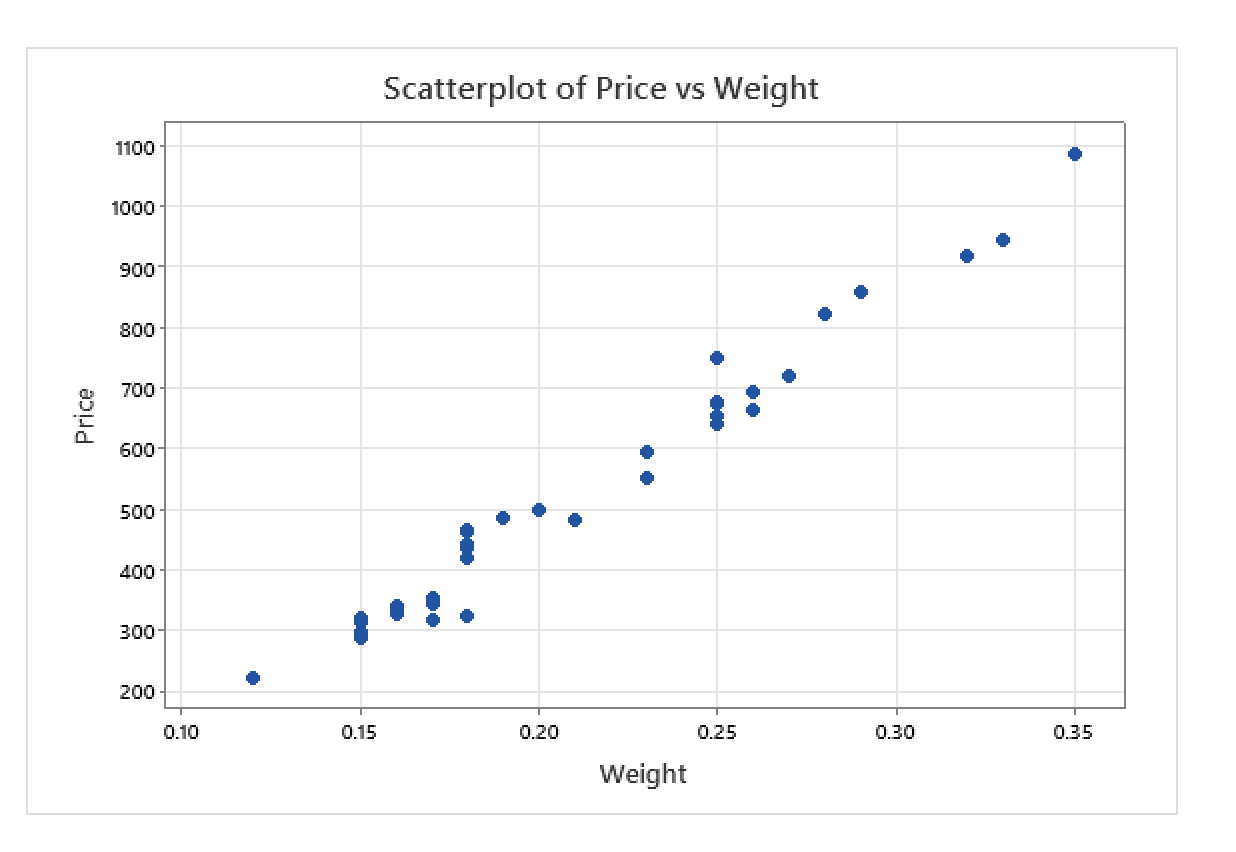
\includegraphics[width=4in]{images/price-weight-scatterplot.png}
\end{center}
\caption{Scatterplot of price (vertical) and weight (horizontal).}
\end{figure}
\item See \autoref{fig:priceweightregression}.
\begin{figure}
\begin{center}
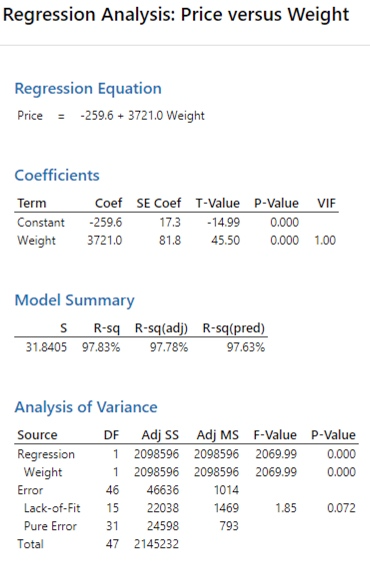
\includegraphics[width=3in]{images/price-weight-regression.png}
\end{center}
\caption{Linear regression analysis for price (response) and weight (predictor).\label{fig:priceweightregression}}
\end{figure}
\item Let $y$ represent the price of a ring and $x$ represent the weight of its diamond. \[y_i=\beta_1x_i+\beta_0+\epsilon_i.\]
\[y_i=b_1x_i+b_0+e_i.\]
\[\hat{y}=(\$3721.00)x-(\$259.60).\]
\item Yes, there is evidence of a significant linear relationship between the price of a ring and the weight of its diamond. The weight coefficient ($\beta_1$) has a Student $t$-statistic of $-14.99$, with a $P$-value of approximately 0.0000. This probability is statistically significant even at the 0.01 percent significance level ($\alpha=0.0001$), indicating that it is very unlikely that the null hypothesis ($H_0:\beta_1=0$) is true. Therefore, there is sufficient evidence to reject the null hypothesis and conclude in favor of the alternative hypothesis ($H_1:\beta_1\neq 0$), that there is in fact a linear relationship between a ring's price and its diamond's weight.
\item On average, for each additional caret a ring's diamond weighs, its price is about \$3721.00 more expensive.
\[t^*=F^{-1}_{46}(0.025)\approx 2.0129\dots\]

We can be ninety-five-percent confident that the true value of $\beta_1$ is in the interval:
\[(\$3556.35,\$3885.65)\]
\item Approximately 97.83 percent of the variation in ring prices can be explained by variations in diamond weight using a least-squares regression line.
\item\[s_e\approx\$31.84\dots\]
\item\[H_0:\beta_1=\$3500.00.\]
\[H_1:\beta_0\neq\$3500.00.\]
\[\alpha=0.01.\]
\[t^*=F^{-1}_{46}(0.005)\approx 2.6870\dots\]
We can be ninety-nine-percent confident that the true value of $\beta_1$ is in this interval
\[(\$3501.20,\$3940.80)\]
Since the value \$3500.00 lies within that interval, there is insufficient evidence to reject the null hypothesis at the one-percent significance level. We cannot conclude beyond a reasonable doubt that the true slope is different from \$3500.00.
\item We can be ninety-five-percent confident that the expected price of rings which weigh 0.230000 carats is in this interval:
\[(\$586.03,\$606.39)\]
\end{enumerate}
\section{Data on stock returns and earnings per share}
\begin{enumerate}
\item It is somewhat unreasonable to fit a linear regression model to these data.

Visually, \autoref{fig:returnepsfittedlineplot} indicates that it is plausible for a negative linear relationship to exist between a company's earnings per share and its stock returns. However, that relationship appears to be extremely weak, and a great deal of error is apparent.

Observation suggests that the underlying assumption that the data are linear may not hold true, and that it is therefore inappropriate to employ a linear regression model.
\begin{figure}[h]
\begin{center}
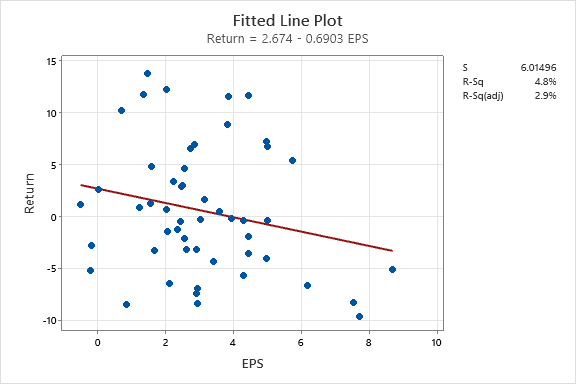
\includegraphics[width=4in]{src/images/return-eps-fitted-line-plot.png}
\end{center}
\caption{Fitted line for return (response) and earnings per share (predictor).\label{fig:returnepsfittedlineplot}}
\end{figure}
\item According to the regression analysis in \autoref{fig:returnepsregression}, the earnings per share metric is not necessarily useful for predicting stock returns.

\[H_0:\beta_1=0.\]
\[H_1:\beta_1\neq 0.\]
\[\alpha=0.05.\]
\[P(t=-1.59\,|\,H_0)\approx 0.118.\]

Since, given that the null hypothesis is true, the probability of obtaining a Student $t$-statistic as extreme as (or more extreme than) $-1.59$ is approximately 11.8 percent, which is greater than the significance level ($\alpha=0.05$), there is insufficient evidence to reject the null hypothesis at the five-percent significance level. We cannot conclude beyond a reasonable doubt that a linear relationship exists between a company's earnings per share and its stock returns.
\begin{figure}[h]
\begin{center}
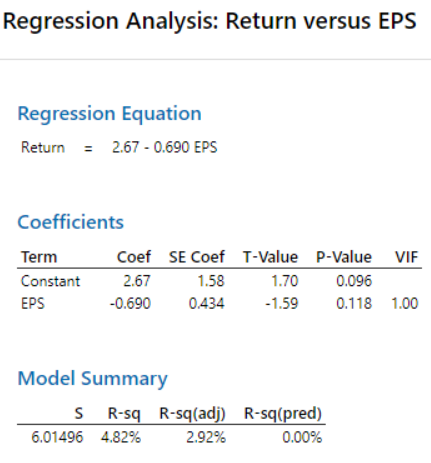
\includegraphics[width=3in]{src/images/return-eps-regression.png}
\end{center}
\caption{Fitted line for return (response) and earnings per share (predictor).\label{fig:returnepsregression}}
\end{figure}
\item Only 4.82 percent of the variation in a company's stock returns can be explained by variations in its earnings per share using a least-squares regression line. This suggests that the linear relationship is very weak.
\item We can be ninety-five-percent confident that the expected stock return of companies with earnings per share of 6 is in this interval:
\[(-13.9263,10.9902)\]
This is not a useful interval: It contains positive values, negative values, and zero. By straddling zero, the interval provides little to no information about whether a stock with earnings per share of 6 offers positive returns, negative returns, or no returns at all. The large margin of error makes this interval even less meaningful.
\end{enumerate}
\end{document}
